
\chapter{Simulations}\label{chapter:simulations}

\begin{itemize}
    \item quickly describe the methodology.
    \item note that both Normalized Exponentiated Gradient and OGA with Lazy Projections behave similary in terms of convergence to equilibria
\end{itemize}

\section{Unique Mixed Nash Equilibrium}\label{section:uniqueMixedNashEquilibrium}

\subsection{Matching Pennies}\label{subsection:machtingPennies}

\begin{table}\centering
\setlength{\extrarowheight}{2pt}
\begin{tabular}{cc|c|c|}
  & \multicolumn{1}{c}{} & \multicolumn{1}{c}{$Heads$}  & \multicolumn{1}{c}{$Tails$} \\\cline{3-4}
  & $Heads$ & $1,-1$ & $-1,1$ \\\cline{3-4}
  & $Tails$ & $-1,1$ & $1,-1$ \\\cline{3-4}
\end{tabular}\caption{\label{tab:payoffMachtingPennies}payoff matrix Matching Pennies}
\end{table}

\begin{itemize}
    \item Note that the MNE is not stable under FTRL as in \ref{section:convergence}. As no strict PNE exists non convergent.
    \item cycling behavior around the MNE.
    \item Empirical frequency converges to MNE as in \cite{jafari}
    \item Similar results in Rock Paper Scissors \ref{subsection:rockPaperScissors}
\end{itemize}

\begin{figure}
    \centering
    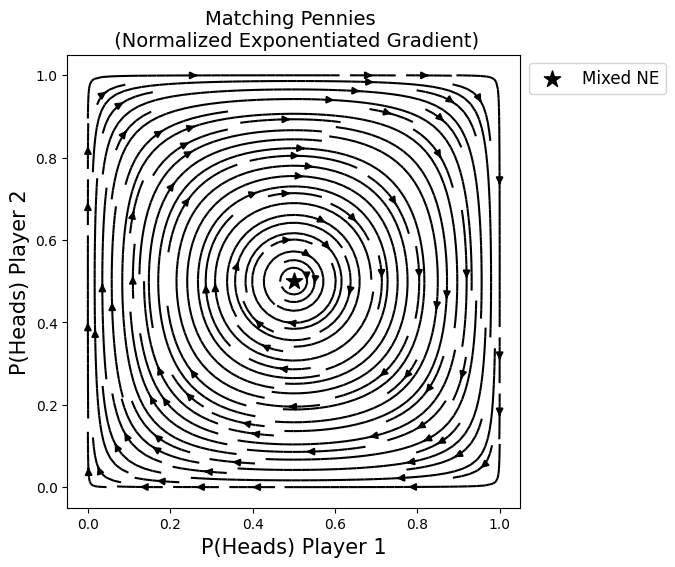
\includegraphics[width=0.5\textwidth]{logos/Pennies1.png}
    \caption{...}
    \label{Pennies1}
\end{figure}

\begin{figure}
    \centering
    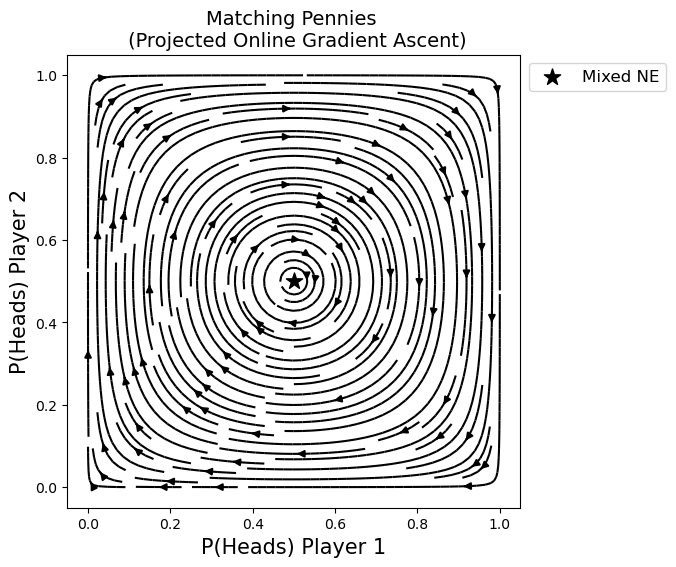
\includegraphics[width=0.5\textwidth]{logos/Pennies2.png}
    \caption{...}
    \label{Pennies2}
\end{figure}

\begin{figure}
    \centering
    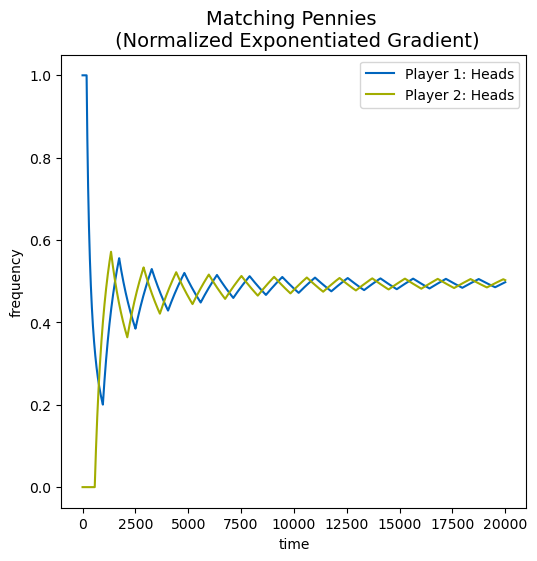
\includegraphics[width=0.5\textwidth]{logos/Pennies3.png}
    \caption{...}
    \label{Pennies3}
\end{figure}


\subsection{Rock Paper Scissors}\label{subsection:rockPaperScissors}

\begin{table}\centering
\setlength{\extrarowheight}{2pt}
\begin{tabular}{cc|c|c|c|}
  & \multicolumn{1}{c}{} & \multicolumn{1}{c}{$Rock$}  & \multicolumn{1}{c}{$Paper$}  & \multicolumn{1}{c}{$Scissors$} \\\cline{3-5}
            & $Rock$ & $0,0$ & $-1,1$ & $1,-1$ \\ \cline{3-5}
            & $Paper$ & $1,-1$ & $0,0$ & $-1,1$ \\\cline{3-5}
            & $Scissors$ & $-1,1$ & $1,-1$ & $0,0$ \\\cline{3-5}
\end{tabular}\caption{\label{tab:payoffRPS}payoff matrix Rock Paper Scissors}
\end{table}

\begin{itemize}
    \item Similar behavior to Matching Pennies. 
    \item Both algorithms cycle but when it come to empirical frequency we see convergence towards the MNE (1/3,1/3,1/3)
\end{itemize}

\begin{figure}
    \centering
    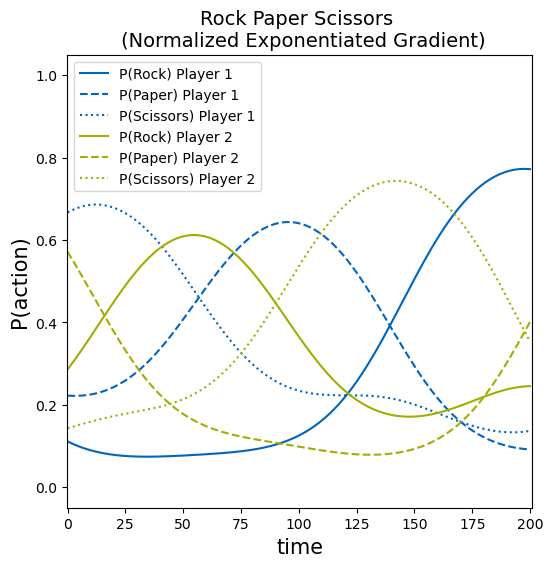
\includegraphics[width=0.5\textwidth]{logos/RPS1.png}
    \caption{...}
    \label{RPS1}
\end{figure}

\begin{figure}
    \centering
    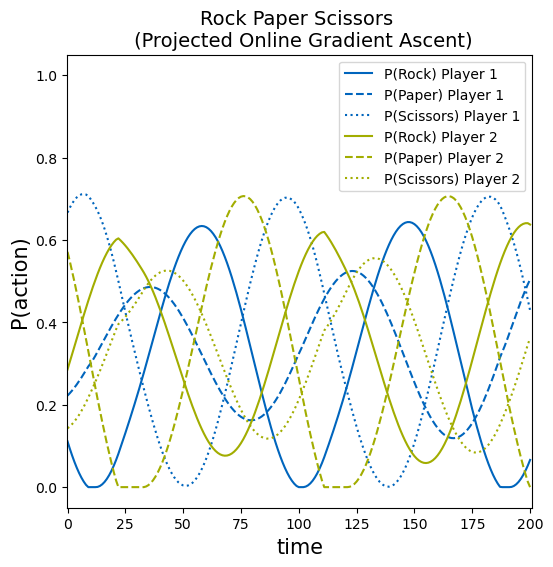
\includegraphics[width=0.5\textwidth]{logos/RPS2.png}
    \caption{...}
    \label{RPS2}
\end{figure}

\begin{figure}
    \centering
    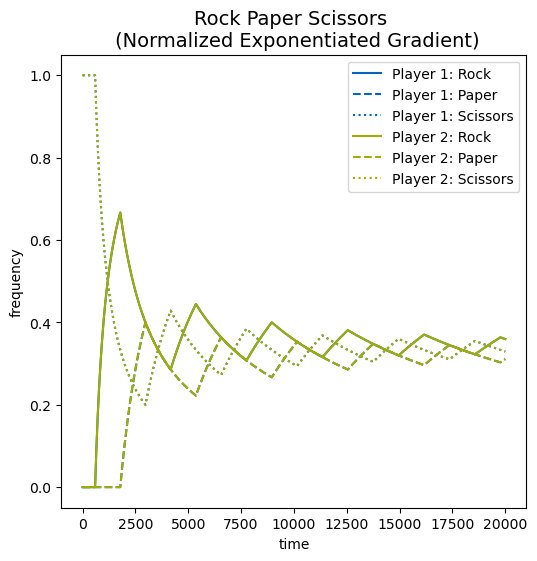
\includegraphics[width=0.5\textwidth]{logos/RPS3.png}
    \caption{...}
    \label{RPS3}
\end{figure}


\subsection{Shapley Game}\label{subsection:shapleyGame}

\begin{table}\centering
\setlength{\extrarowheight}{2pt}
\begin{tabular}{cc|c|c|c|}
  & \multicolumn{1}{c}{} & \multicolumn{1}{c}{$L$}  & \multicolumn{1}{c}{$C$}  & \multicolumn{1}{c}{$R$} \\\cline{3-5}
            & $T$ & $1,0$ & $0,1$ & $0,0$ \\ \cline{3-5}
            & $M$ & $0,0$ & $1,0$ & $0,1$ \\\cline{3-5}
            & $B$ & $0,1$ & $0,0$ & $1,0$ \\\cline{3-5}
\end{tabular}\caption{\label{tab:payoffShapley}payoff matrix Shapley Game}
\end{table}

\begin{itemize}
    \item no convergence of both algorithms
    \item cycles grow exponentially
    \item also no convergence in empirical frequency even though same MNE as in Rock Paper Scissors
    \item related to the fact that not this game is not zero sum \cite{jafari} p.6
\end{itemize}

\begin{figure}
    \centering
    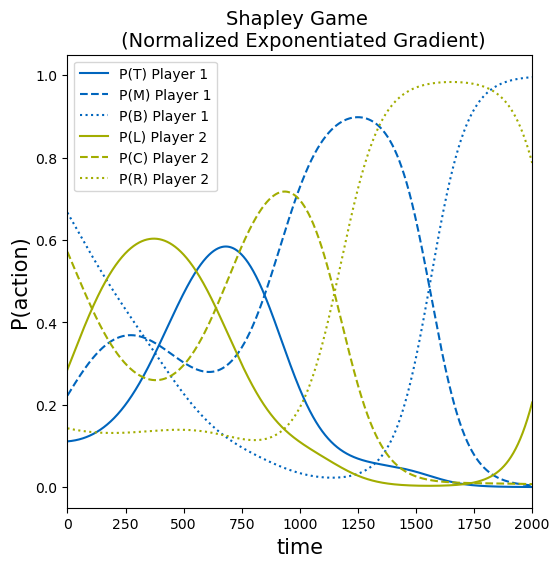
\includegraphics[width=0.5\textwidth]{logos/Shapley1.png}
    \caption{...}
    \label{Shapley1}
\end{figure}

\begin{figure}
    \centering
    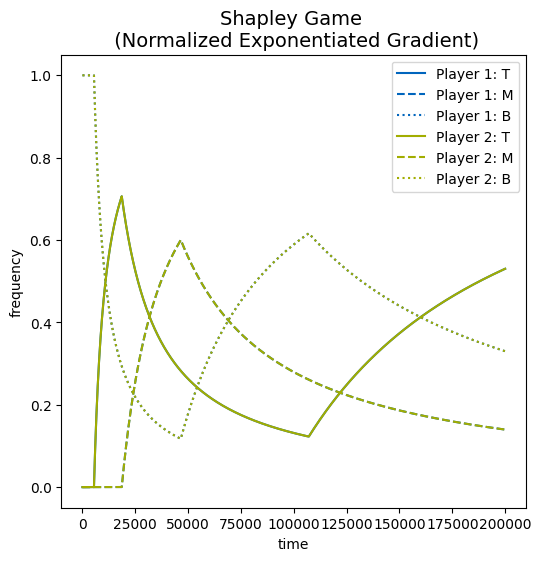
\includegraphics[width=0.5\textwidth]{logos/Shapley2.png}
    \caption{...}
    \label{Shapley2}
\end{figure}



\section{Unique Pure Nash Equilibrium}\label{section:uniquePureNashEquilibrium}

\subsection{Prisoner's Dilemma}\label{subsection:prisonersDilemma}

\begin{table}\centering
\setlength{\extrarowheight}{2pt}
\begin{tabular}{cc|c|c|}
  & \multicolumn{1}{c}{} & \multicolumn{1}{c}{$Silent$}  & \multicolumn{1}{c}{$Betray$} \\\cline{3-4}
  & $Silent$ & $-1,-1$ & $-3,0$ \\\cline{3-4}
  & $Betray$ & $0,-3$ & $-2,-2$ \\\cline{3-4}
\end{tabular}\caption{\label{tab:payoffPrisoners}payoff matrix Prisoner's Dilemma}
\end{table}

\begin{itemize}
    \item If x* globally stable then x* is unique NE from \ref{section:convergence}
    \item both algorithms converge globally to the strict PNE
    \item show figure where x* is globally stable
\end{itemize}

\begin{figure}
    \centering
    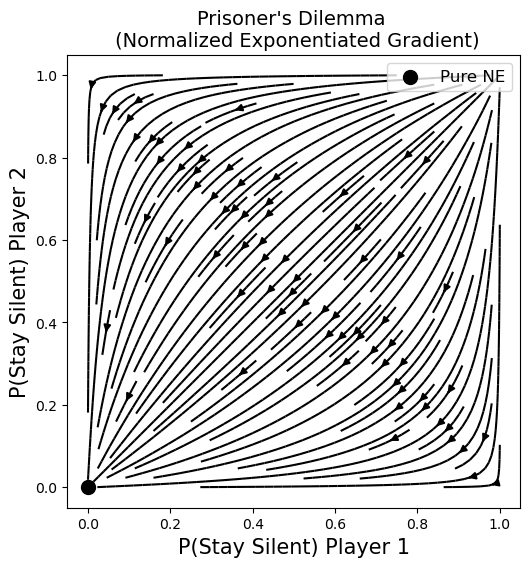
\includegraphics[width=0.5\textwidth]{logos/Prisoners1.png}
    \caption{...}
    \label{Prisoners1}
\end{figure}

\begin{figure}
    \centering
    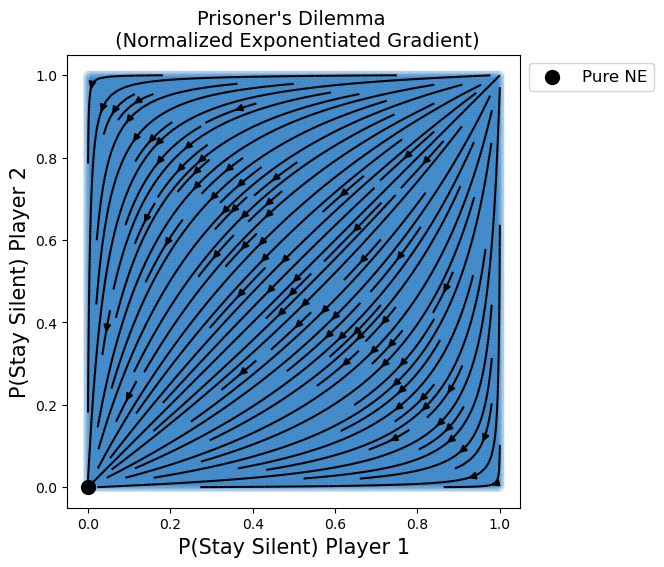
\includegraphics[width=0.5\textwidth]{logos/Prisoners2.png}
    \caption{...}
    \label{Prisoners2}
\end{figure}

\begin{figure}
    \centering
    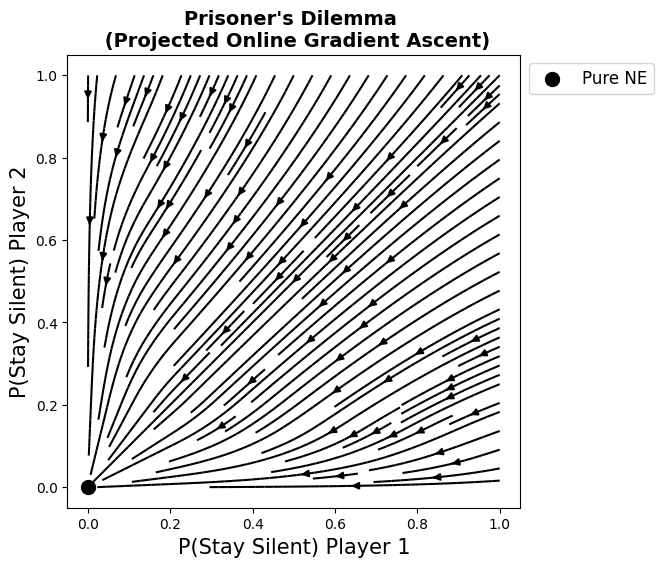
\includegraphics[width=0.5\textwidth]{logos/Prisoners3.png}
    \caption{...}
    \label{Prisoners3}
\end{figure}


\section{Multiple Pure Nash Equilibria}\label{section:multiplePureNashEquilibria}

\subsection{Coordination Game}\label{subsection:coordinationGame}

\begin{table}\centering
\setlength{\extrarowheight}{2pt}
\begin{tabular}{cc|c|c|c|}
  & \multicolumn{1}{c}{} & \multicolumn{1}{c}{$L$}  & \multicolumn{1}{c}{$C$}  & \multicolumn{1}{c}{$R$} \\\cline{3-5}
            & $T$ & $3,3$ & $0,0$ & $0,0$ \\ \cline{3-5}
            & $M$ & $0,0$ & $2,2$ & $0,2$ \\\cline{3-5}
            & $B$ & $0,0$ & $0,0$ & $1,1$ \\\cline{3-5}
\end{tabular}\caption{\label{tab:payoffCoordination3x3}payoff matrix Coordination Game}
\end{table}

\begin{itemize}
    \item non zero sum does not imply non convergence as the shapley game is suggesting
    \item this game converges to one of the three PNE in every case
    \item most of the time both algorithms converge to the pareto optimal PNE similar as in \cite{jafari}
    \item the convergence to the other PNE also occurs but less often.
    \item I haven't found the pattern on when this game converges to a specific PNE
\end{itemize}

\begin{figure}
    \centering
    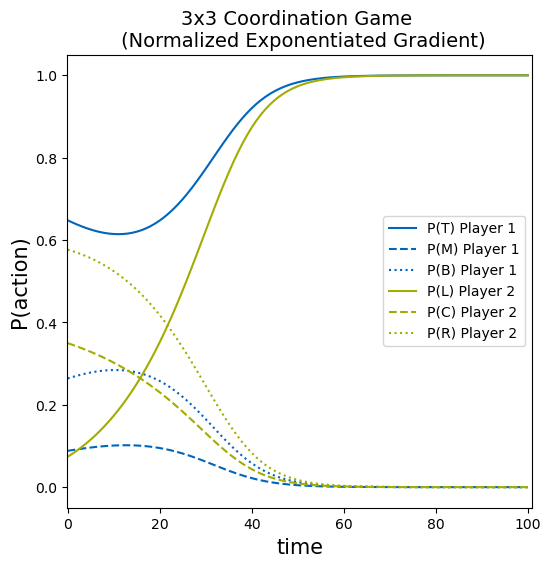
\includegraphics[width=0.5\textwidth]{logos/Coordination3x3-1.png}
    \caption{...}
    \label{Coordination3x3-1}
\end{figure}

\begin{figure}
    \centering
    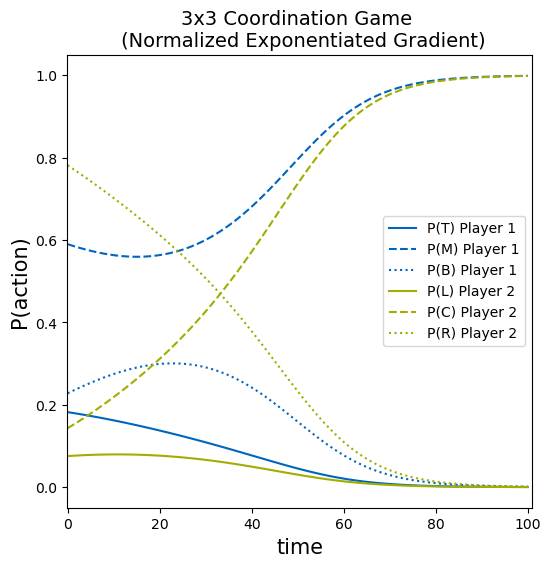
\includegraphics[width=0.5\textwidth]{logos/Coordination3x3-2.png}
    \caption{...}
    \label{Coordination3x3-2}
\end{figure}

\begin{figure}
    \centering
    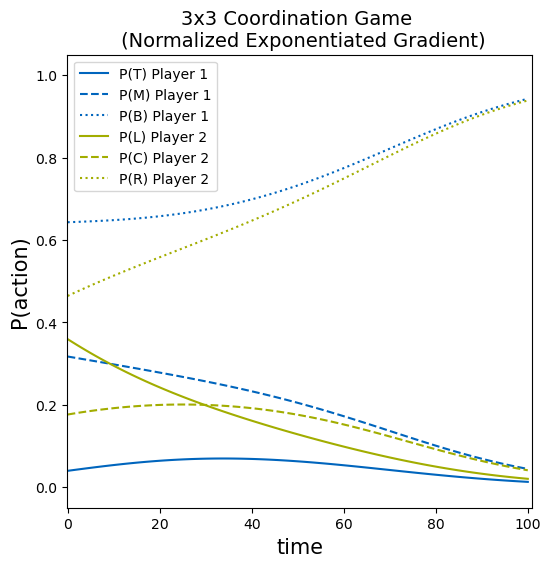
\includegraphics[width=0.5\textwidth]{logos/Coordination3x3-3.png}
    \caption{...}
    \label{Coordination3x3-3}
\end{figure}


\section{Mixed and Pure Nash Equilibria}\label{section:MixedandPureNashEquilibria}

\subsection{Battle Of Sexes}\label{subsection:battleOfSexes}

\begin{table}\centering
\setlength{\extrarowheight}{2pt}
\begin{tabular}{cc|c|c|}
  & \multicolumn{1}{c}{} & \multicolumn{1}{c}{$Fight$}  & \multicolumn{1}{c}{$Ballet$} \\\cline{3-4}
  & $Fight$ & $3,2$ & $0,0$ \\\cline{3-4}
  & $Ballet$ & $0,0$ & $2,3$ \\\cline{3-4}
\end{tabular}\caption{\label{tab:payoffBattleOfSexes}payoff matrix Battle of Sexes}
\end{table}

\begin{itemize}
    \item Again MNE is not stable
    \item both PNE are strict as in \ref{section:equilibriaConcepts}
    \item convergence locally of both PNE, since both are locally stable
    \item as mentioned in \ref{section:convergence} stable equilibria are locally attracting with high probability \cite{mertikopoulos}, Abstract, Theorem 4.11 (local convergence of local stable equilibria with high probability) 
\end{itemize}

\begin{figure}
    \centering
    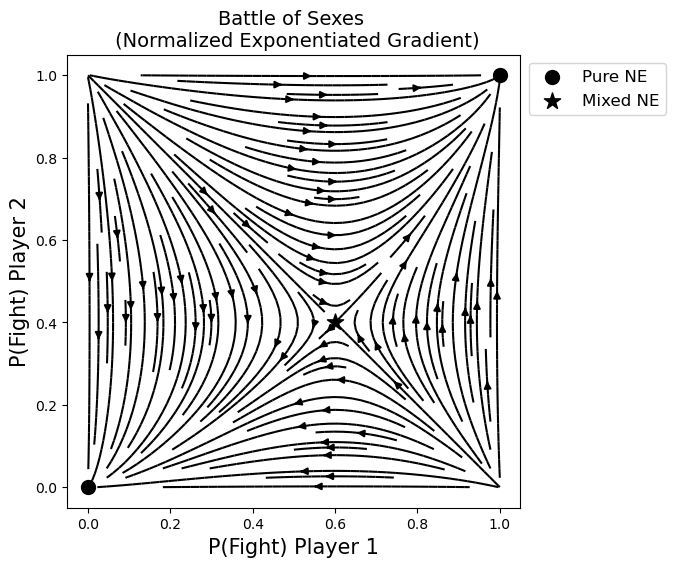
\includegraphics[width=0.5\textwidth]{logos/BattleOfSexes1.png}
    \caption{...}
    \label{BattleOfSexes1}
\end{figure}

\begin{figure}
    \centering
    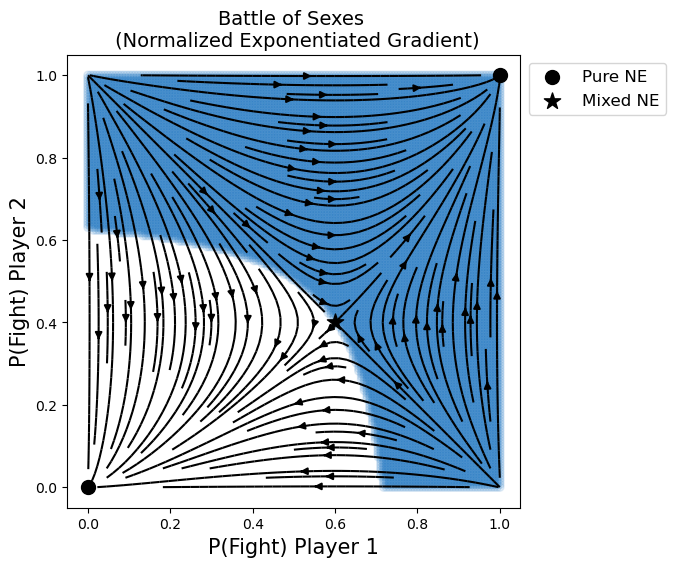
\includegraphics[width=0.5\textwidth]{logos/BattleOfSexes2.png}
    \caption{...}
    \label{BattleOfSexes2}
\end{figure}

\begin{figure}
    \centering
    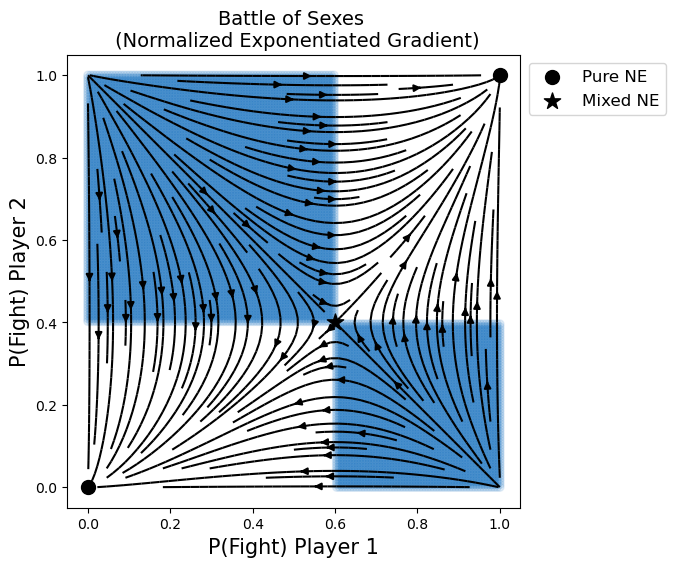
\includegraphics[width=0.5\textwidth]{logos/BattleOfSexes3.png}
    \caption{...}
    \label{BattleOfSexes3}
\end{figure}

\begin{figure}
    \centering
    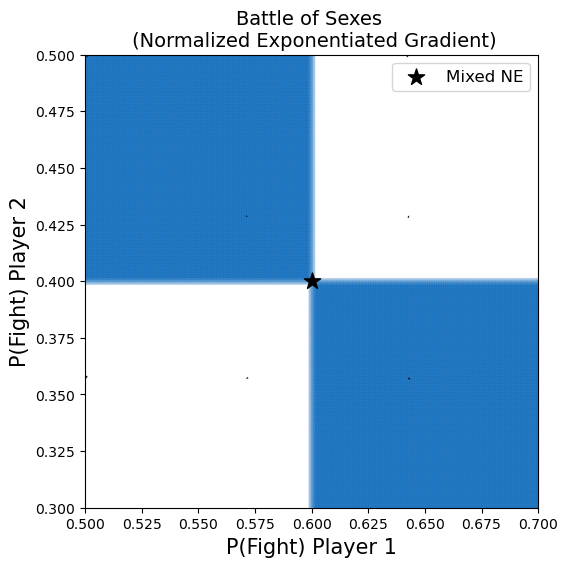
\includegraphics[width=0.5\textwidth]{logos/BattleOfSexes4.png}
    \caption{...}
    \label{BattleOfSexes4}
\end{figure}

\begin{figure}
    \centering
    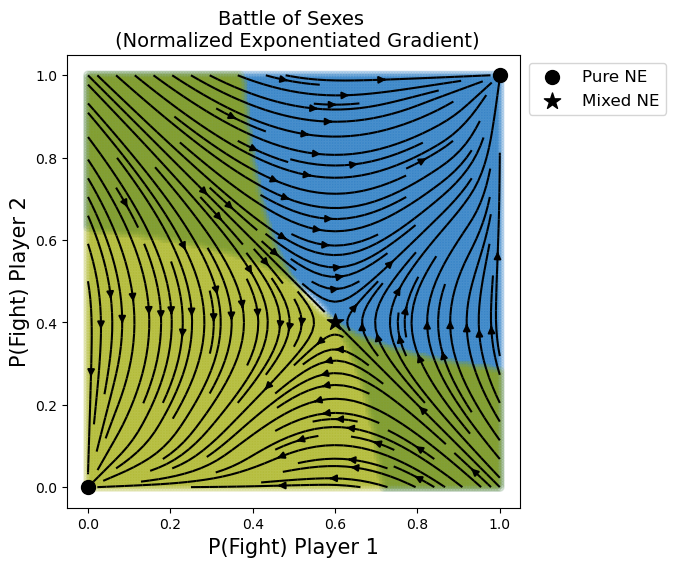
\includegraphics[width=0.5\textwidth]{logos/BattleOfSexes5.png}
    \caption{...}
    \label{BattleOfSexes5}
\end{figure}


\subsection{Intersection Game}\label{subsection:intersectionGame}

\begin{table}\centering
\setlength{\extrarowheight}{2pt}
\begin{tabular}{cc|c|c|}
  & \multicolumn{1}{c}{} & \multicolumn{1}{c}{$Stop$}  & \multicolumn{1}{c}{$Go$} \\\cline{3-4}
  & $Stop$ & $0,0$ & $0,1$ \\\cline{3-4}
  & $Go$ & $1,0$ & $-100,-100$ \\\cline{3-4}
\end{tabular}\caption{\label{tab:payoffIntersection}payoff matrix Intersection Game}
\end{table}

\begin{itemize}
    \item similar results as in Battle of Sexes \ref{subsection:battleOfSexes}
    \item figures might be misleading. It looks like the algorithm converges to the MNE but looking a a specific trajectory one can see that they converge to the PNEs only
    \item maybe show figure where both stable regions intersect
    \item again convergence to both PNEs as both are locally stable 
    \item shall I leave it out?
\end{itemize}

\begin{figure}
    \centering
    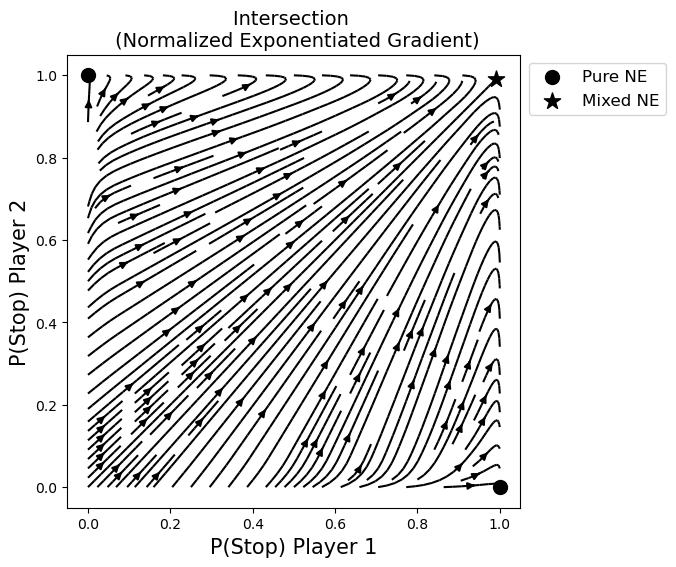
\includegraphics[width=0.5\textwidth]{logos/Intersection1.png}
    \caption{...}
    \label{Intersection1}
\end{figure}

\begin{figure}
    \centering
    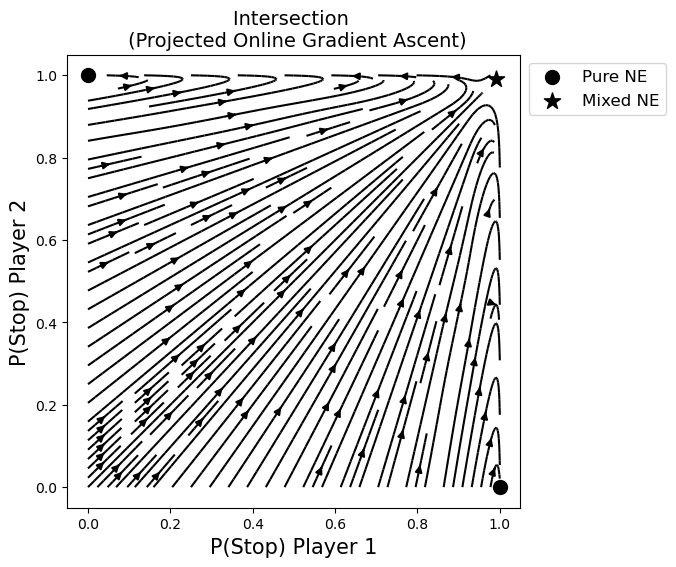
\includegraphics[width=0.5\textwidth]{logos/Intersection2.png}
    \caption{...}
    \label{Intersection2}
\end{figure}

\begin{figure}
    \centering
    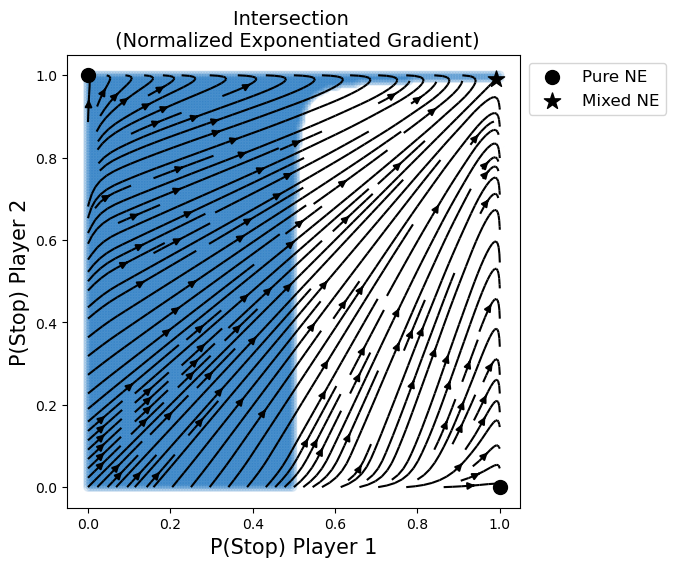
\includegraphics[width=0.5\textwidth]{logos/Intersection3.png}
    \caption{...}
    \label{Intersection3}
\end{figure}

\begin{figure}
    \centering
    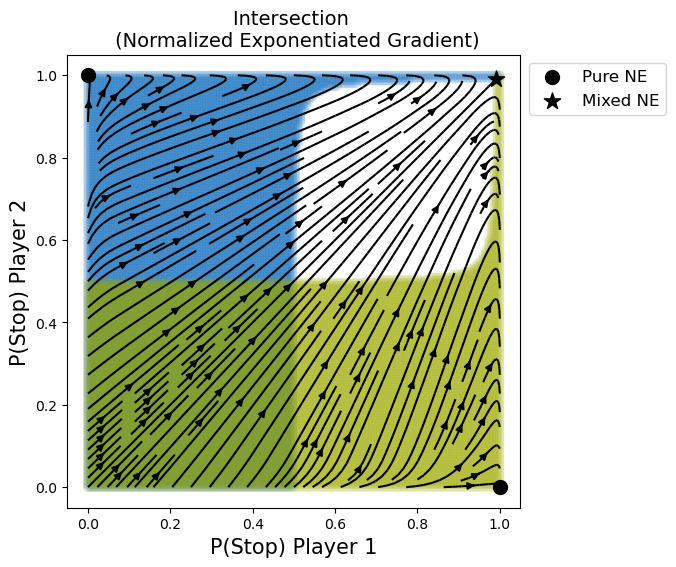
\includegraphics[width=0.5\textwidth]{logos/Intersection4.png}
    \caption{...}
    \label{Intersection4}
\end{figure}

\begin{figure}
    \centering
    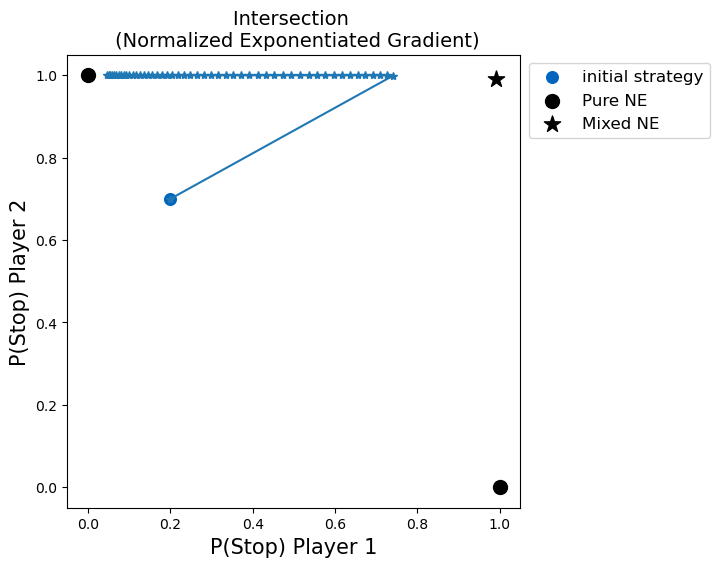
\includegraphics[width=0.5\textwidth]{logos/Intersection5.png}
    \caption{...}
    \label{Intersection5}
\end{figure}

\begin{figure}
    \centering
    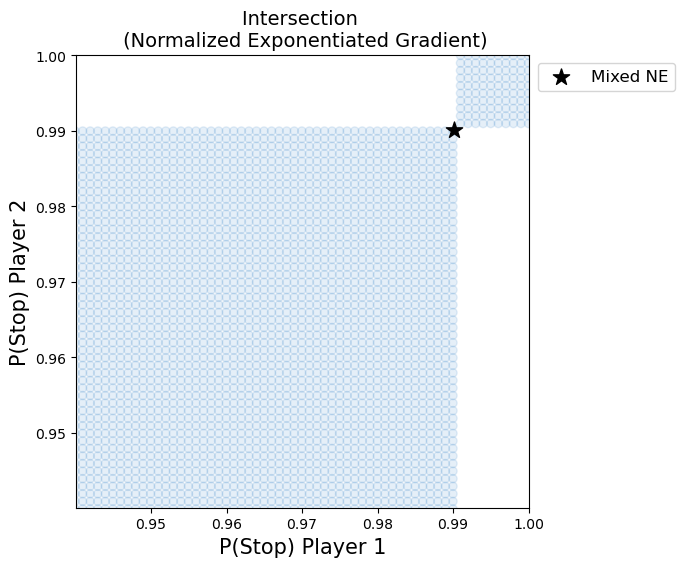
\includegraphics[width=0.5\textwidth]{logos/Intersection6.png}
    \caption{...}
    \label{Intersection6}
\end{figure}


\section{Weak Nash Equilibria}\label{section:WeakNashEquilibria}

\subsection{2x2}\label{subsection:2x2}

\begin{table}\centering
\setlength{\extrarowheight}{2pt}
\begin{tabular}{cc|c|c|}
  & \multicolumn{1}{c}{} & \multicolumn{1}{c}{$H$}  & \multicolumn{1}{c}{$T$} \\\cline{3-4}
  & $H$ & $2,3$ & $1,2$ \\\cline{3-4}
  & $T$ & $1,2$ & $2,2$ \\\cline{3-4}
\end{tabular}\caption{\label{tab:payoffStrictAndWeak2x2}payoff matrix Strict and Weak Nash Equilibria 2x2}
\end{table}

\begin{itemize}
    \item quickly explain the game and why there is both a strict and a weak NE according to \ref{section:equilibriaConcepts}
    \item Note that the plots are misleading as the trajectory stays within the simplex but for some initial points
    it diverges towards the "left wall". 
    \item Still both algorithms never converge towards the weak NE
    \item When getting numerically close to the weak NE it get unstable, i.e variational stability is positive
    \item Unclear how to interpret \cite{flokas} Flokas Theorem 2 
    \item The weak NE seems to disrupt the convergence to the strict NE. 
    \item As the strictly NE is locally stable it is locally attracting (but definitely not globally)
\end{itemize}

\begin{figure}
    \centering
    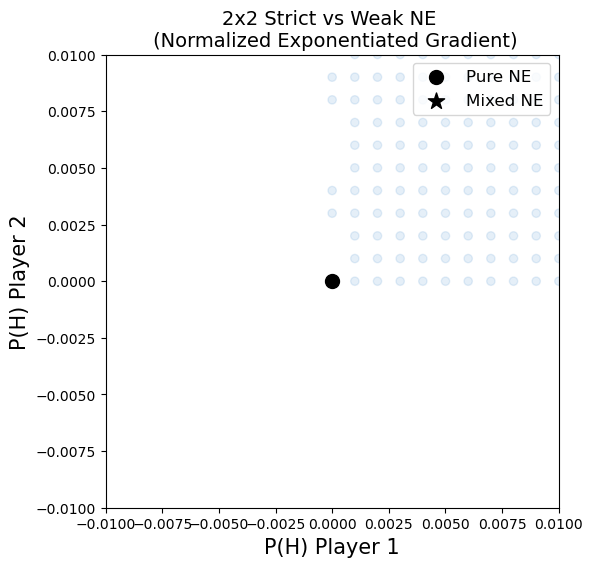
\includegraphics[width=0.5\textwidth]{logos/Weak1.png}
    \caption{...}
    \label{Weak1}
\end{figure}

\begin{figure}
    \centering
    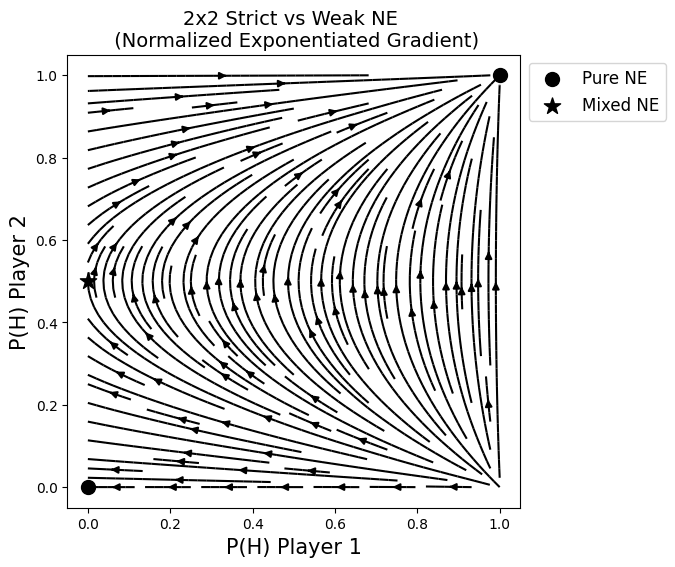
\includegraphics[width=0.5\textwidth]{logos/Weak2.png}
    \caption{...}
    \label{Weak2}
\end{figure}

\begin{figure}
    \centering
    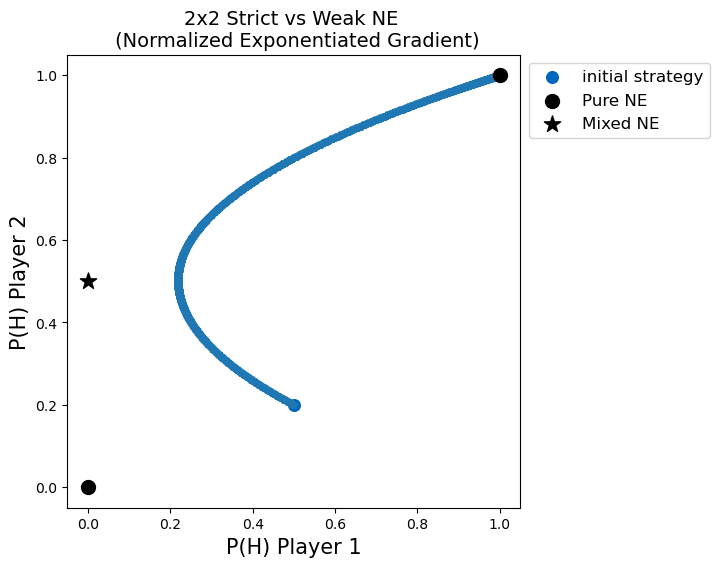
\includegraphics[width=0.5\textwidth]{logos/Weak3.png}
    \caption{...}
    \label{Weak3}
\end{figure}

\begin{figure}
    \centering
    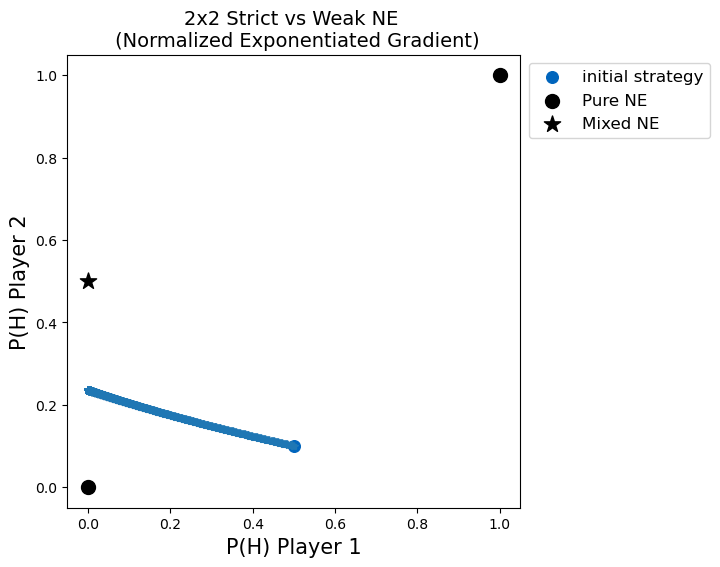
\includegraphics[width=0.5\textwidth]{logos/Weak4.png}
    \caption{...}
    \label{Weak4}
\end{figure}

\begin{figure}
    \centering
    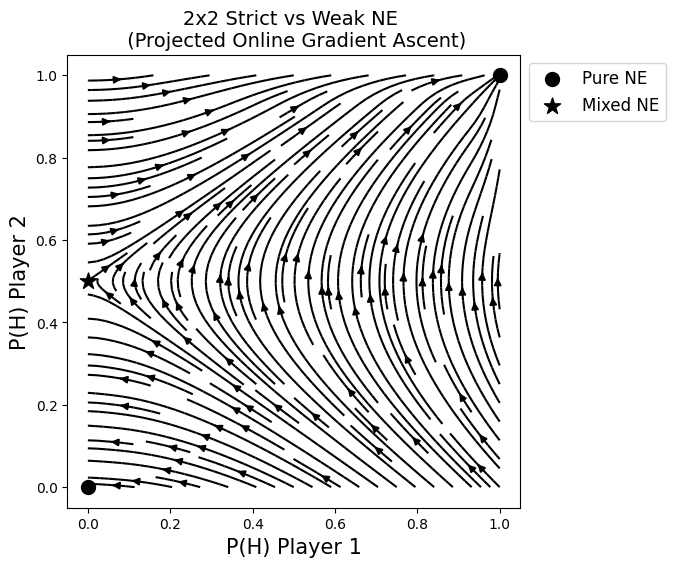
\includegraphics[width=0.5\textwidth]{logos/Weak5.png}
    \caption{...}
    \label{Weak5}
\end{figure}

\begin{figure}
    \centering
    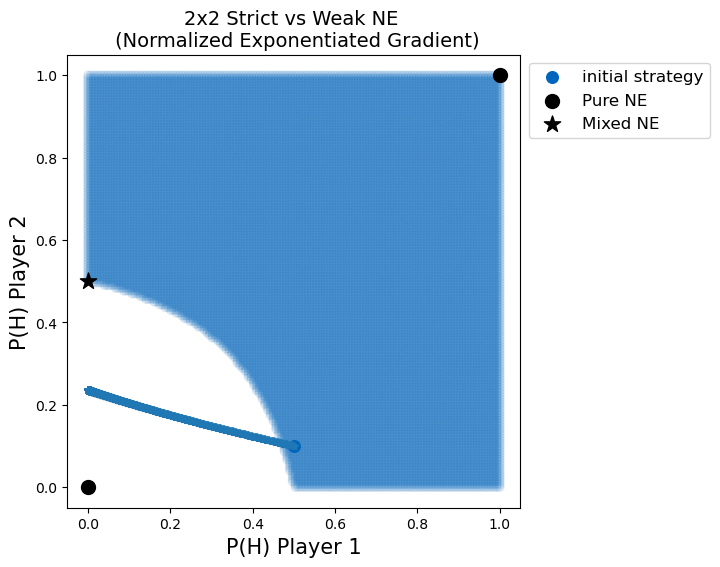
\includegraphics[width=0.5\textwidth]{logos/Weak6.png}
    \caption{...}
    \label{Weak6}
\end{figure}


\subsection{3x3}\label{subsection:3x3}

\begin{table}\centering
\setlength{\extrarowheight}{2pt}
\begin{tabular}{cc|c|c|c|}
  & \multicolumn{1}{c}{} & \multicolumn{1}{c}{$A$}  & \multicolumn{1}{c}{$B$}  & \multicolumn{1}{c}{$C$} \\\cline{3-5}
            & $X$ & $2,3$ & $1,2$ & $1,1$ \\ \cline{3-5}
            & $Y$ & $1,1$ & $2,1$ & $3,2$ \\\cline{3-5}
            & $Z$ & $1,2$ & $2,2$ & $2,1$ \\\cline{3-5}
\end{tabular}\caption{\label{tab:payoffStrictAndWeak3x3}payoff matrix Strict and Weak Nash Equilibria 3x3}
\end{table}

\begin{itemize}
    \item Always converging towards Strict PNE (X,A), (Y,C)
    \item Never converging to the Weak PNE (Y,B)
\end{itemize}

\begin{figure}
    \centering
    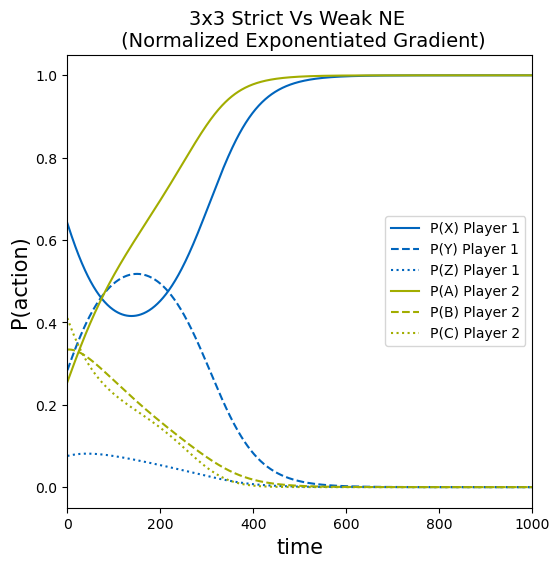
\includegraphics[width=0.5\textwidth]{logos/Weak3x3-1.png}
    \caption{...}
    \label{Weak3x3-1}
\end{figure}

\begin{figure}
    \centering
    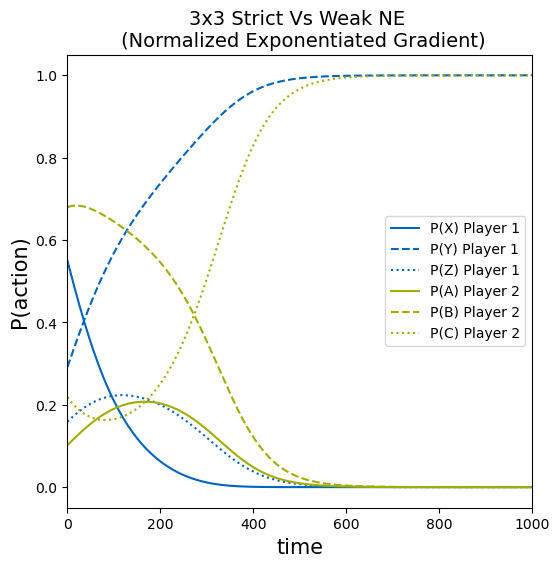
\includegraphics[width=0.5\textwidth]{logos/Weak3x3-2.png}
    \caption{...}
    \label{Weak3x3-2}
\end{figure}
